\documentclass{standalone}
\usepackage{tikz}
\usetikzlibrary{patterns, positioning}
\usepackage[sfdefault]{ClearSans} %% option 'sfdefault' activates Clear Sans as the default text font
\usepackage[T1]{fontenc}

\begin{document}
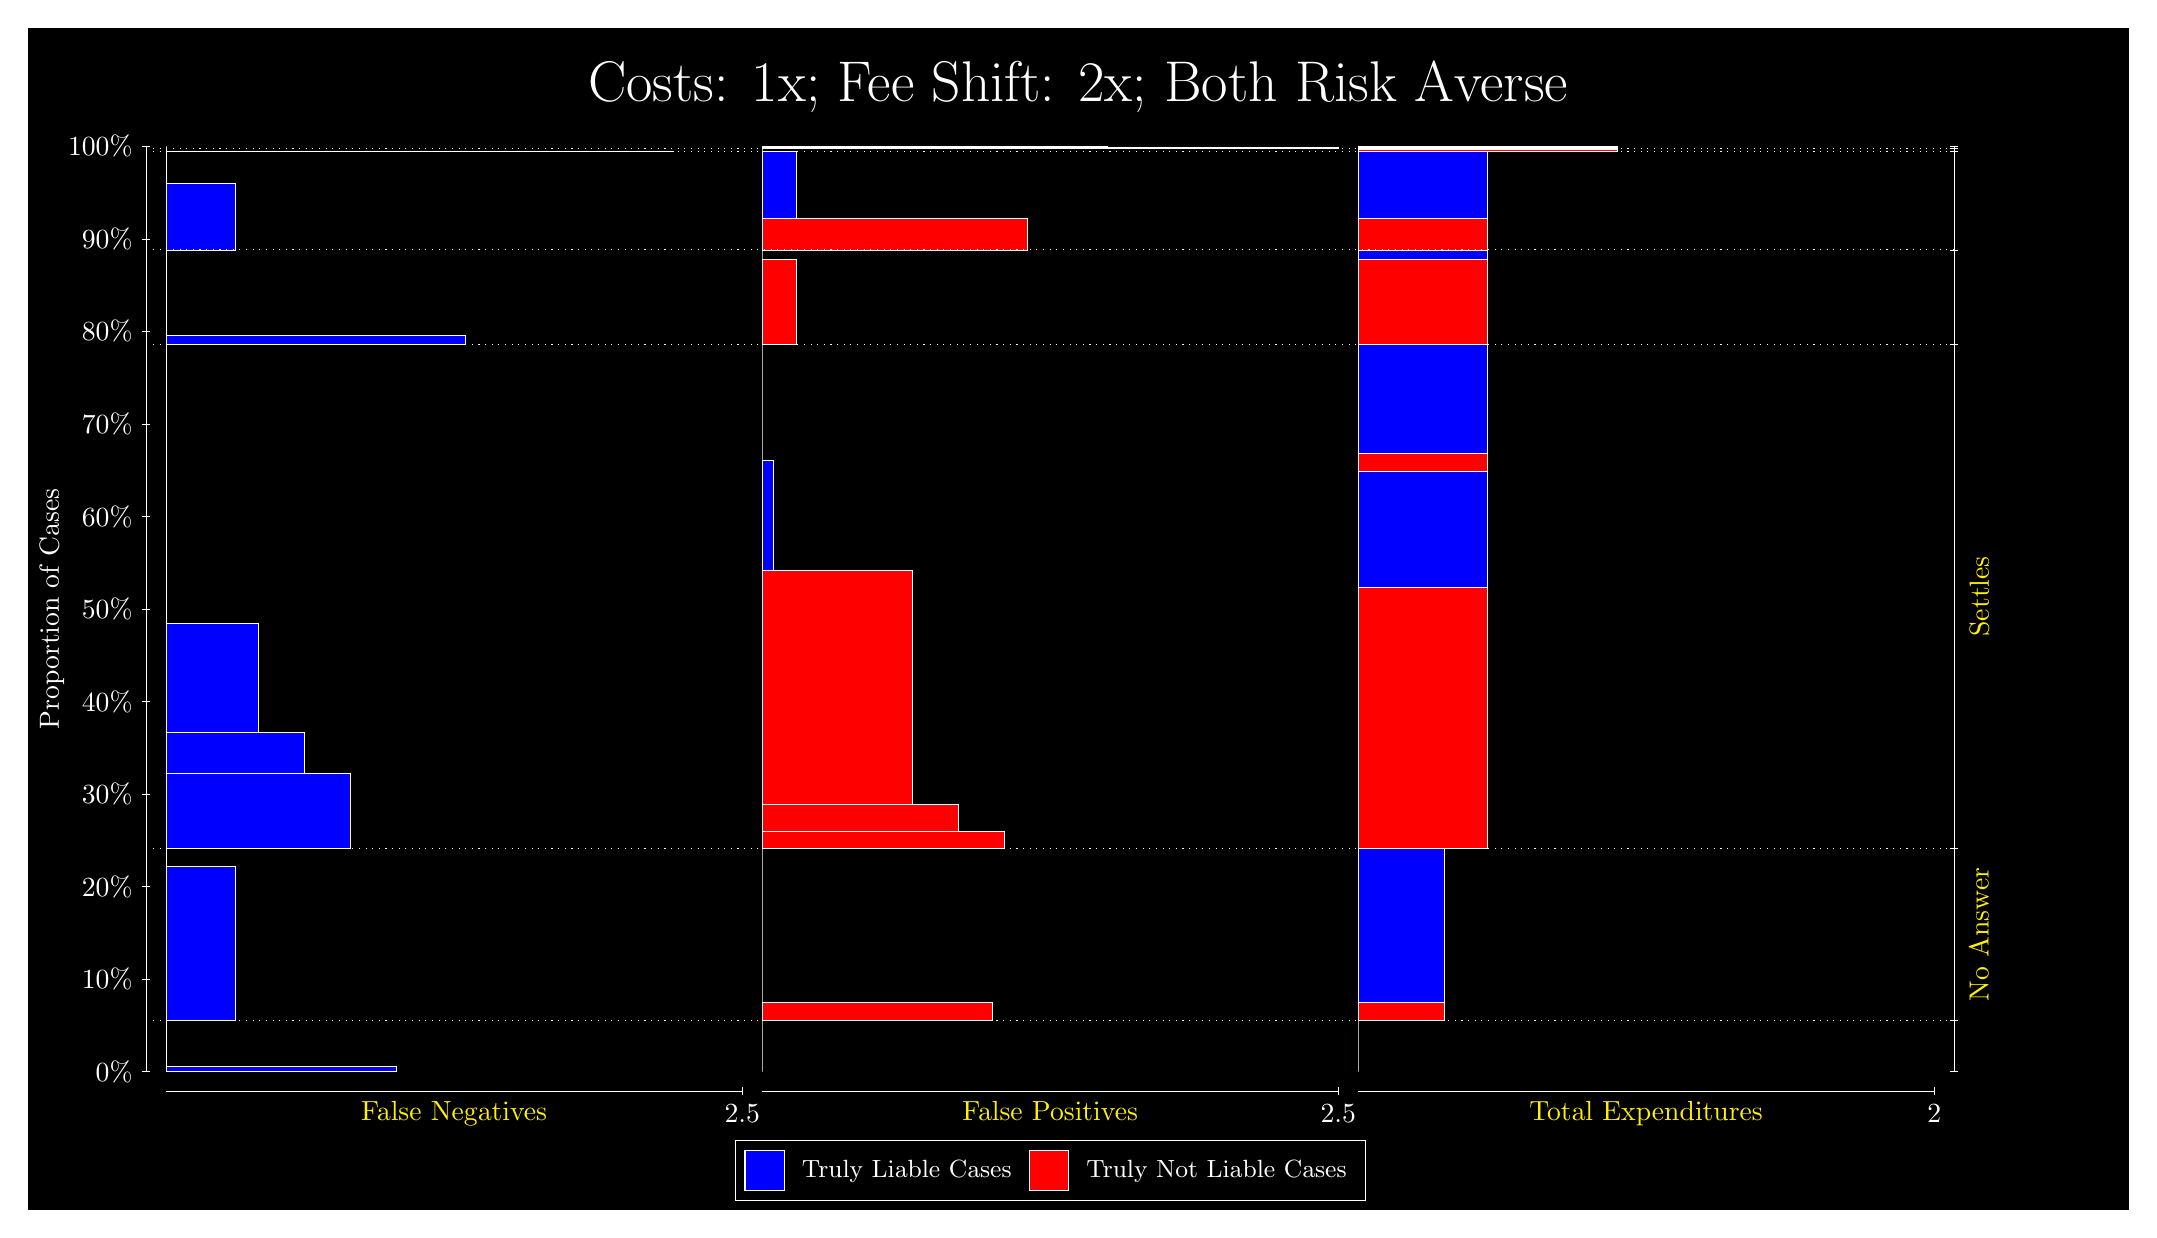
\begin{tikzpicture}
\draw[fill=black] (0,0) rectangle (26.667,15);
\draw[text=white] (0,13.5) rectangle (26.667,15) node[midway] {\huge Costs: 1x; Fee Shift: 2x; Both Risk Averse};
\draw[white, very thin] (1.5,1.75) -- (1.5,13.5);
\node[rotate=90, text=white, anchor=center] at (0.3, 7.625) {Proportion of Cases};
\draw[white, very thin] (1.45,1.75) -- (1.55,1.75);
\node[text=white, anchor=east] at (1.45, 1.75) {0\%};
\draw[white, very thin] (1.45,2.925) -- (1.55,2.925);
\node[text=white, anchor=east] at (1.45, 2.925) {10\%};
\draw[white, very thin] (1.45,4.1) -- (1.55,4.1);
\node[text=white, anchor=east] at (1.45, 4.1) {20\%};
\draw[white, very thin] (1.45,5.275) -- (1.55,5.275);
\node[text=white, anchor=east] at (1.45, 5.275) {30\%};
\draw[white, very thin] (1.45,6.45) -- (1.55,6.45);
\node[text=white, anchor=east] at (1.45, 6.45) {40\%};
\draw[white, very thin] (1.45,7.625) -- (1.55,7.625);
\node[text=white, anchor=east] at (1.45, 7.625) {50\%};
\draw[white, very thin] (1.45,8.8) -- (1.55,8.8);
\node[text=white, anchor=east] at (1.45, 8.8) {60\%};
\draw[white, very thin] (1.45,9.975) -- (1.55,9.975);
\node[text=white, anchor=east] at (1.45, 9.975) {70\%};
\draw[white, very thin] (1.45,11.15) -- (1.55,11.15);
\node[text=white, anchor=east] at (1.45, 11.15) {80\%};
\draw[white, very thin] (1.45,12.325) -- (1.55,12.325);
\node[text=white, anchor=east] at (1.45, 12.325) {90\%};
\draw[white, very thin] (1.45,13.5) -- (1.55,13.5);
\node[text=white, anchor=east] at (1.45, 13.5) {100\%};

\draw[white, very thin] (24.457,1.75) -- (24.457,13.5);
\draw[white, very thin] (24.407,1.75) -- (24.507,1.75);
\node[anchor=west] at (24.407, 1.75) {};
\draw[white, very thin] (24.407,2.4005) -- (24.507,2.4005);
\node[anchor=west] at (24.407, 2.4005) {};
\draw[white, very thin] (24.407,4.582) -- (24.507,4.582);
\node[anchor=west] at (24.407, 4.582) {};
\draw[white, very thin] (24.407,10.987) -- (24.507,10.987);
\node[anchor=west] at (24.407, 10.987) {};
\draw[white, very thin] (24.407,12.184) -- (24.507,12.184);
\node[anchor=west] at (24.407, 12.184) {};
\draw[white, very thin] (24.407,13.432) -- (24.507,13.432);
\node[anchor=west] at (24.407, 13.432) {};
\draw[white, very thin] (24.407,13.477) -- (24.507,13.477);
\node[anchor=west] at (24.407, 13.477) {};
\draw[white, very thin] (24.407,13.5) -- (24.507,13.5);
\node[anchor=west] at (24.407, 13.5) {};

\draw[white, very thin, fill=blue] (1.75,1.75) rectangle (4.6775,1.8184);
\draw[white, very thin, fill=red] (1.75,1.8184) rectangle (1.75,2.4005);
\draw[white, very thin, fill=blue] (1.75,2.4005) rectangle (2.6283,4.3543);
\draw[white, very thin, fill=red] (1.75,4.3543) rectangle (1.75,4.582);
\draw[white, very thin, fill=blue] (1.75,4.582) rectangle (4.092,5.5368);
\draw[white, very thin, fill=blue] (1.75,5.5368) rectangle (3.5065,6.0575);
\draw[white, very thin, fill=blue] (1.75,6.0575) rectangle (2.921,7.4485);
\draw[white, very thin, fill=red] (1.75,7.4485) rectangle (1.75,10.987);
\draw[white, very thin, fill=blue] (1.75,10.987) rectangle (5.5558,11.105);
\draw[white, very thin, fill=red] (1.75,11.105) rectangle (1.75,12.184);
\draw[white, very thin, fill=blue] (1.75,12.184) rectangle (2.6283,13.029);
\draw[white, very thin, fill=red] (1.75,13.029) rectangle (1.75,13.432);
\draw[white, very thin, fill=blue] (1.75,13.432) rectangle (8.1906,13.443);
\draw[white, very thin, fill=red] (1.75,13.443) rectangle (1.75,13.477);
\draw[white, very thin, fill=red] (1.75,13.477) rectangle (1.75,13.488);
\draw[white, very thin, fill=blue] (1.75,13.488) rectangle (1.75,13.5);
\draw[white, very thin, fill=red] (9.3189,1.75) rectangle (9.3189,2.3321);
\draw[white, very thin, fill=blue] (9.3189,2.3321) rectangle (9.3189,2.4005);
\draw[white, very thin, fill=red] (9.3189,2.4005) rectangle (12.246,2.6282);
\draw[white, very thin, fill=blue] (9.3189,2.6282) rectangle (9.3189,4.582);
\draw[white, very thin, fill=red] (9.3189,4.582) rectangle (12.393,4.8021);
\draw[white, very thin, fill=red] (9.3189,4.8021) rectangle (11.807,5.1402);
\draw[white, very thin, fill=red] (9.3189,5.1402) rectangle (11.222,8.121);
\draw[white, very thin, fill=blue] (9.3189,8.121) rectangle (9.4652,9.512);
\draw[white, very thin, fill=blue] (9.3189,9.512) rectangle (9.3189,10.987);
\draw[white, very thin, fill=red] (9.3189,10.987) rectangle (9.758,12.066);
\draw[white, very thin, fill=blue] (9.3189,12.066) rectangle (9.3189,12.184);
\draw[white, very thin, fill=red] (9.3189,12.184) rectangle (12.686,12.587);
\draw[white, very thin, fill=blue] (9.3189,12.587) rectangle (9.758,13.432);
\draw[white, very thin, fill=red] (9.3189,13.432) rectangle (9.3189,13.466);
\draw[white, very thin, fill=blue] (9.3189,13.466) rectangle (9.3189,13.477);
\draw[white, very thin, fill=red] (9.3189,13.477) rectangle (16.638,13.488);
\draw[white, very thin, fill=blue] (9.3189,13.488) rectangle (13.71,13.5);
\draw[white, very thin, fill=red] (16.888,1.75) rectangle (16.888,2.3321);
\draw[white, very thin, fill=blue] (16.888,2.3321) rectangle (16.888,2.4005);
\draw[white, very thin, fill=red] (16.888,2.4005) rectangle (17.986,2.6282);
\draw[white, very thin, fill=blue] (16.888,2.6282) rectangle (17.986,4.582);
\draw[white, very thin, fill=red] (16.888,4.582) rectangle (18.534,7.9009);
\draw[white, very thin, fill=blue] (16.888,7.9009) rectangle (18.534,9.3763);
\draw[white, very thin, fill=red] (16.888,9.3763) rectangle (18.534,9.5964);
\draw[white, very thin, fill=blue] (16.888,9.5964) rectangle (18.534,10.987);
\draw[white, very thin, fill=red] (16.888,10.987) rectangle (18.534,12.066);
\draw[white, very thin, fill=blue] (16.888,12.066) rectangle (18.534,12.184);
\draw[white, very thin, fill=red] (16.888,12.184) rectangle (18.534,12.587);
\draw[white, very thin, fill=blue] (16.888,12.587) rectangle (18.534,13.432);
\draw[white, very thin, fill=red] (16.888,13.432) rectangle (20.181,13.466);
\draw[white, very thin, fill=blue] (16.888,13.466) rectangle (20.181,13.477);
\draw[white, very thin, fill=red] (16.888,13.477) rectangle (20.181,13.488);
\draw[white, very thin, fill=blue] (16.888,13.488) rectangle (20.181,13.5);
\draw[white, dotted] (1.5,2.4005) -- (24.457,2.4005);
\draw[white, dotted] (1.5,4.582) -- (24.457,4.582);
\draw[white, dotted] (1.5,10.987) -- (24.457,10.987);
\draw[white, dotted] (1.5,12.184) -- (24.457,12.184);
\draw[white, dotted] (1.5,13.432) -- (24.457,13.432);
\draw[white, dotted] (1.5,13.477) -- (24.457,13.477);
\draw[white, very thin] (1.75,1.5) -- (9.0689,1.5);
\node[text=yellow, anchor=north] at (5.4094, 1.5) {False Negatives};
\draw[white, very thin] (9.0689,1.45) -- (9.0689,1.55);
\node[text=white, anchor=north] at (9.0689, 1.45) {2.5};

\draw[white, very thin] (9.3189,1.5) -- (16.638,1.5);
\node[text=yellow, anchor=north] at (12.978, 1.5) {False Positives};
\draw[white, very thin] (16.638,1.45) -- (16.638,1.55);
\node[text=white, anchor=north] at (16.638, 1.45) {2.5};

\draw[white, very thin] (16.888,1.5) -- (24.207,1.5);
\node[text=yellow, anchor=north] at (20.547, 1.5) {Total Expenditures};
\draw[white, very thin] (24.207,1.45) -- (24.207,1.55);
\node[text=white, anchor=north] at (24.207, 1.45) {2};


\node[text=yellow, centered, rotate=90] at (24.777, 3.4913) {No Answer};
\node[text=yellow, centered, rotate=90] at (24.777, 7.7847) {Settles};





\draw (12.978300999999998,1.5) node[draw=none] (baseCoordinate) {};
\begin{scope}[align=center]
        \matrix[scale=0.5, draw=white, below=0.5cm of baseCoordinate, nodes={draw}, column sep=0.1cm]{
            \node[rectangle, draw, minimum width=0.5cm, minimum height=0.5cm, fill=blue] {}; &
            \node[draw=none, font=\small, text=white] (B) {Truly Liable Cases}; &
            \node[rectangle, draw, minimum width=0.5cm, minimum height=0.5cm, fill=red] {}; &
            \node[draw=none, font=\small, text=white] (B) {Truly Not Liable Cases}; \\
            };
\end{scope}

\end{tikzpicture}
\end{document}